%!TEX root = ../uwo.tex

\begin{frame}[plain,noframenumbering]
	\centering
	\vspace*{2.6cm}
	\Huge \colorit{Part I}
	\vskip 20pt
	\Large Hyperharmonic analysis
\end{frame}

\begin{frame}{Complex systems}

	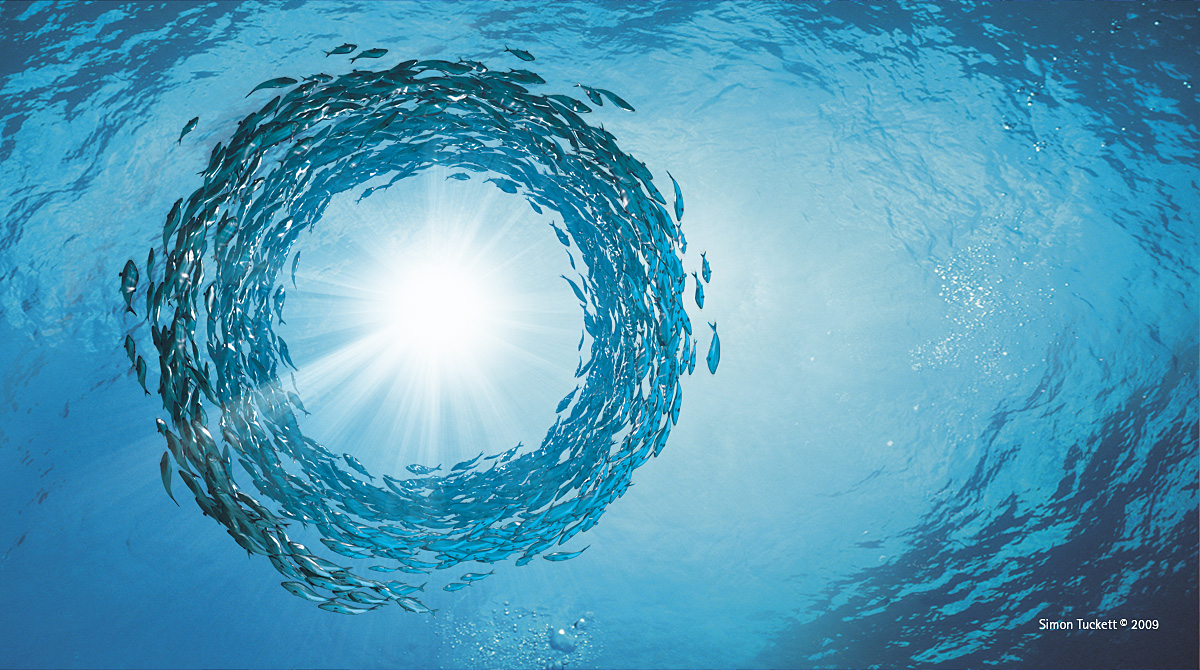
\includegraphics[scale=.23]{aux/fishes}

	\bigskip
	\textit{The whole is greater than the sum of its parts.}

	\pause\vskip 10pt
	\colorit{Question}: How to \colorit{quantify} this slogan?
\end{frame}

\begin{frame}{Information signals}
	\pause
	Let $X_0, \dots, X_N$ be probability distributions

	\vskip 5pt

	\begin{itemize}
		\pause\item The \colorit{entropy} of each
		\[
		\textstyle H(X_i) = - \sum_{x_i} p(x_i) \log p(x_i).
		\]
		\vspace*{-20pt}\pause\item The \colorit{mutual information} of pairs
		\[
		I(X; Y) = H(X, Y) - H(X \mid Y) - H(Y \mid X).
		\]
		\vspace*{-20pt}\pause\item The \colorit{interaction information} of triples
		\begin{align*}
			I(X;Y;Z) &=
			H(X) + H(Y) + H(Z) \\
			& - H(X,Y) - H(X,Z) - H(Y,Z) \\
			& + H(X,Y,Z).
		\end{align*}
		\vspace*{-20pt}\pause\item \colorit{Analogues} for higher cardinality subsets.
	\end{itemize}

	\vskip 10pt
	\pause

	\colorit{Problem:} Number of subsets \colorit{grows exponentially} with $N$.
\end{frame}

\begin{frame}{Simplicial complex}

	\begin{center}
		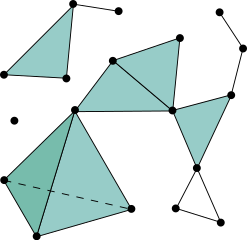
\includegraphics[scale=.35]{aux/simplicial_complex}
	\end{center}

	\pause
	Weighted with \colorit{structural} information. (e.g. EEG node positions)

	\pause\medskip
	Signals are the same as $\R$ valued \colorit{cochains}. E.g.

	\qquad Entropy : 0-cochain \\
	\qquad Mutual information : 1-cochain \\
	\qquad Interaction information : 2-cochain \\
	\qquad Higher order signals : $n$-cochains
%	\hspace*{2cm}$\vdots$

	\pause\medskip
	\colorit{Boundary} $\partial_n$ (incidence matrix) and \colorit{coboundary} $\delta_n$ (adjoint operator),\\
	\smallskip
	Both \colorit{act} on cochains.
\end{frame}

\begin{frame}{Hyperharmonic analysis}
	\pause
	\colorit{Analogy:} Listen to a few harmonics to tell a guitar and a~piano apart.

	\pause\bigskip
	\colorit{Contribution (Med.--Rosas--Rodr\'iguez--Cofr\'e)}\\
	A principled method to compress high-order information signals based on Fourier analysis and combinatorial topology.

	\pause\bigskip
	\colorit{Fourier basis:} Eigenvectors of the \colorit{discrete Laplacian}
	\[
	\displaystyle{L_n = \partial_{n+1} \delta_n + \delta_{n-1} \partial_{n}}.
	\]

	\pause\medskip
	How to measure \colorit{compressibility}?

	\pause\medskip
	Give signal $\alpha$, let $\{\alpha_i\}$ be its coeff's in a basis with $\alpha_1^2 \geq \alpha_2^2 \geq \cdots$
	\begin{equation*}
		\text{EV}_{\alpha}(k) = \frac{ \alpha_k^2}{{\displaystyle \sum_{i} \alpha_i^2}}
		\qquad \text{ and } \qquad
		\text{CEV}_{\alpha}(k) = \sum_{1\leq i \leq k} \text{EV}_{\alpha}(i),
	\end{equation*}
\end{frame}

\begin{frame}{Proof of concept: Haydn's symphonies}
	\pause\vskip -5pt
	Music as a probability distribution.

	\pause\vskip 5pt
	We analyzed two high-order information signals across four dimensions:% O-info and S-info.

	\pause\vskip 7pt
	\hspace*{-15pt}
	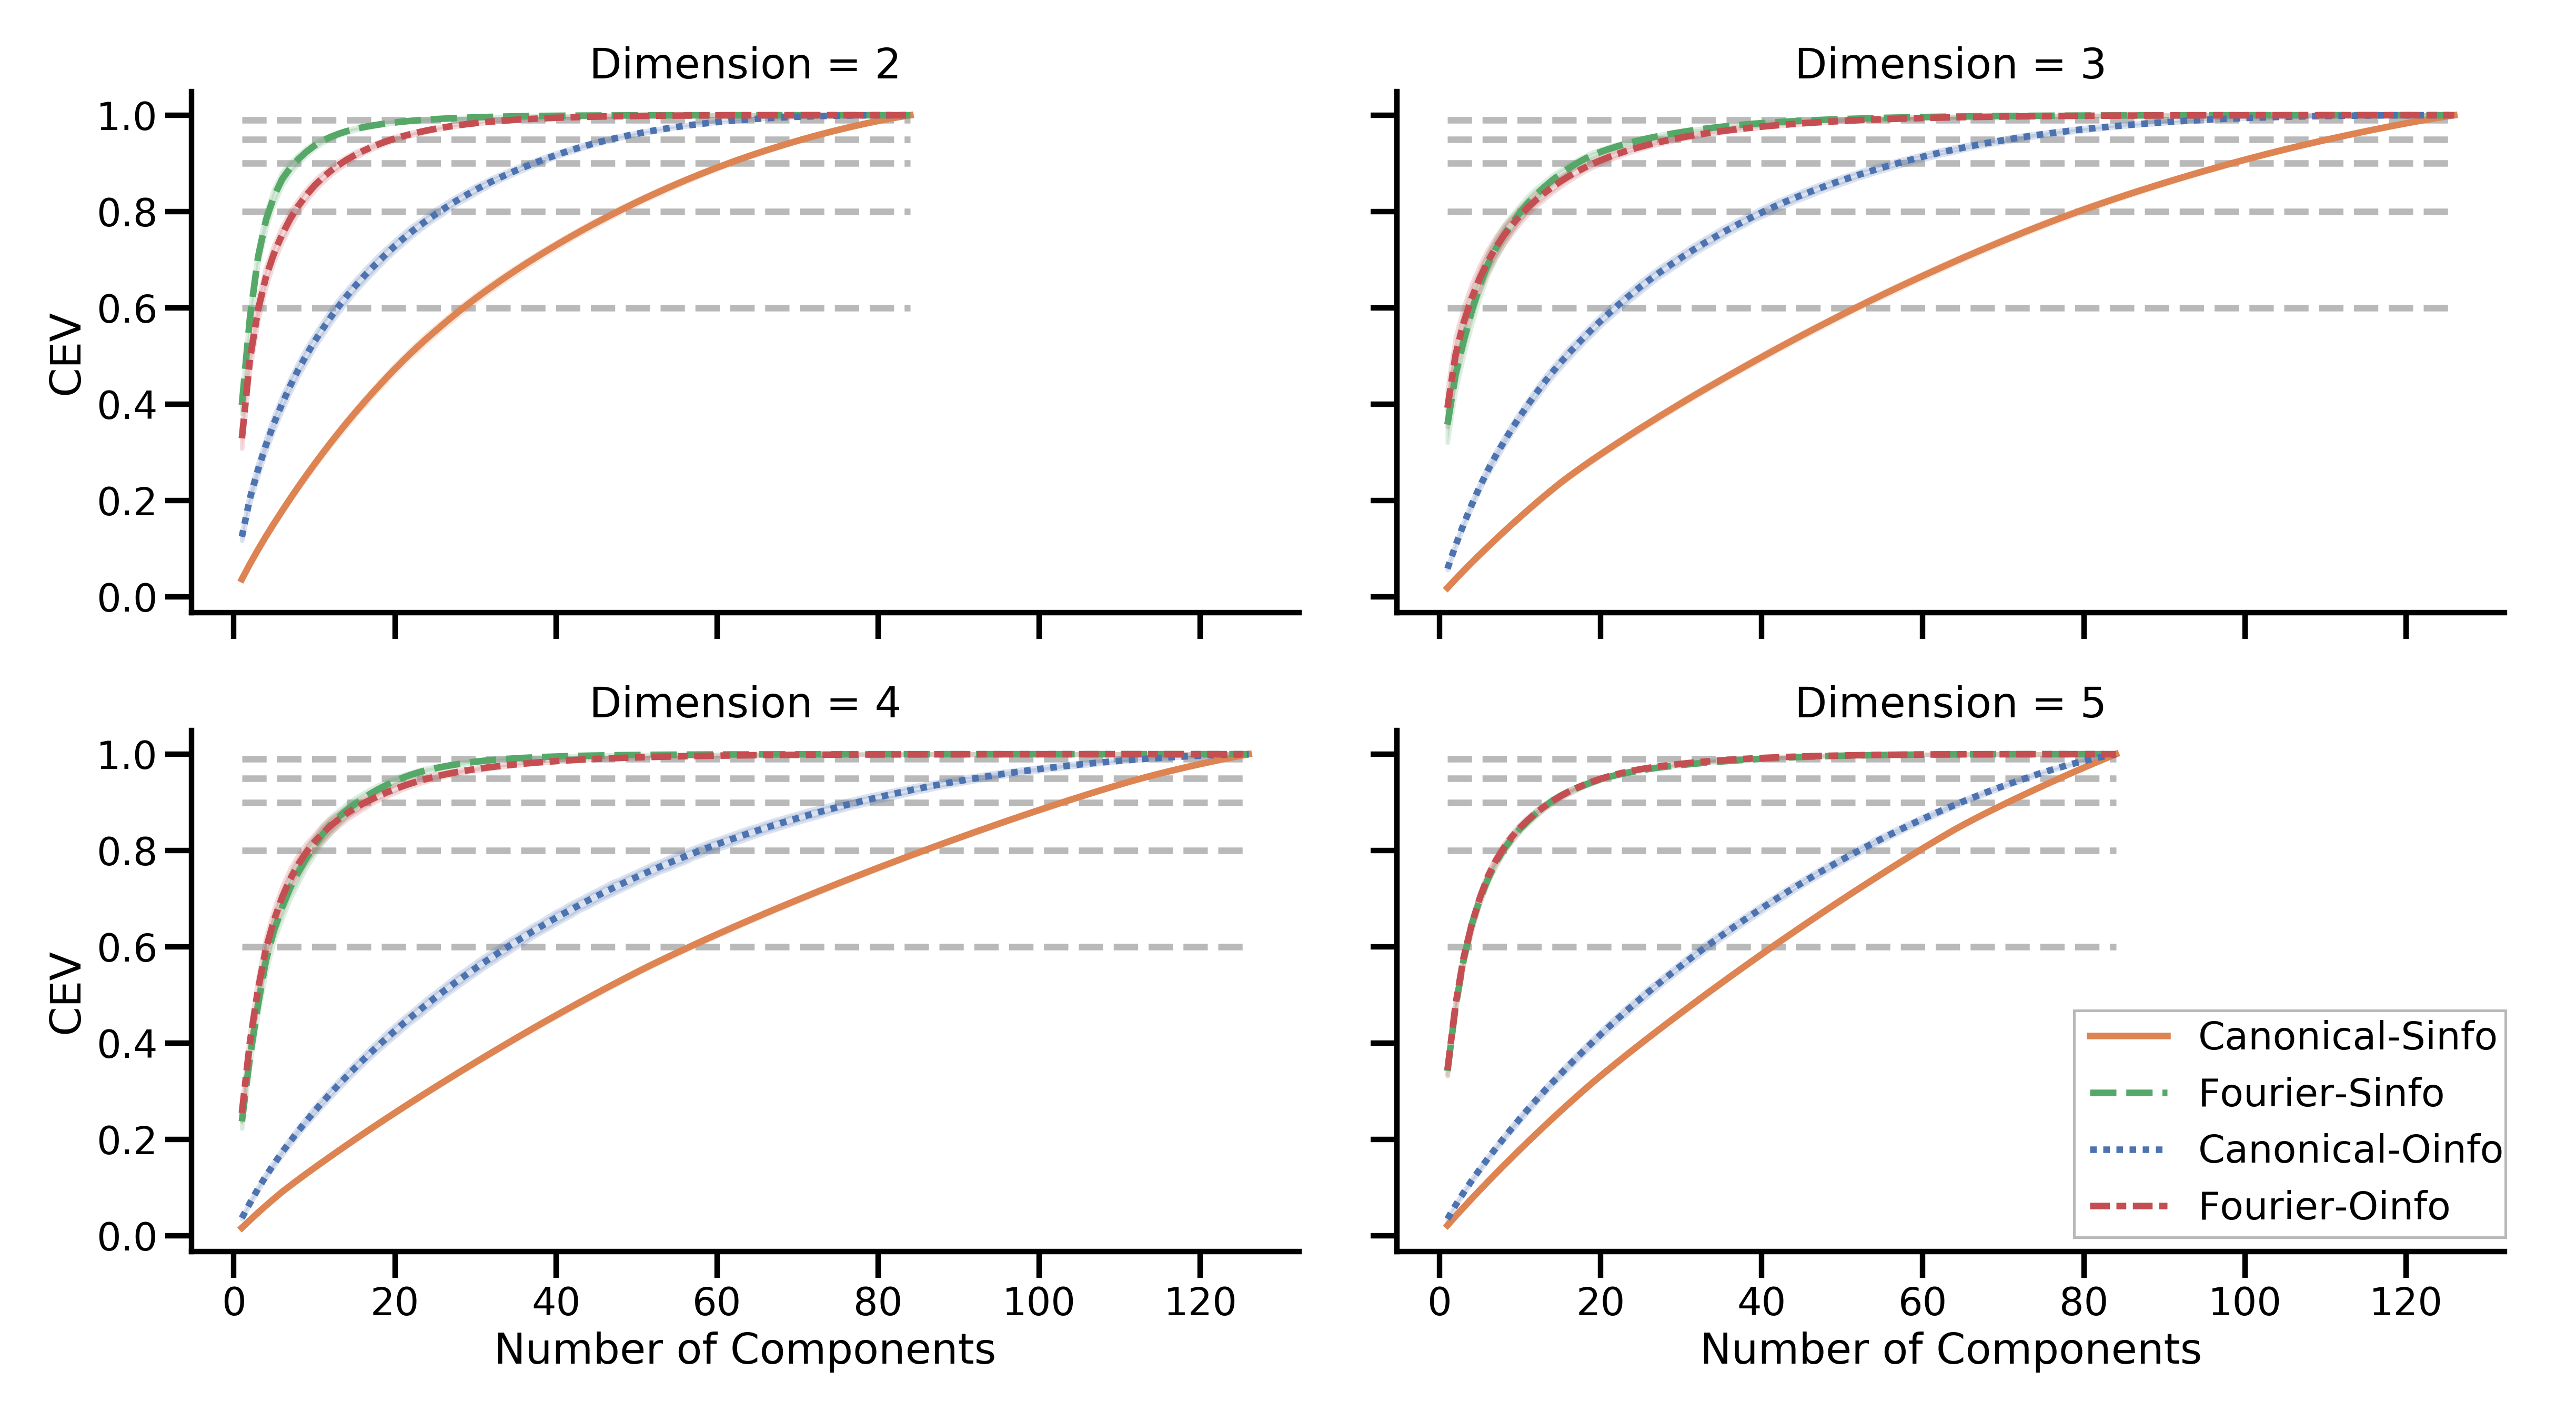
\includegraphics[scale=.096]{aux/hyperharmonic}
\end{frame}